% chktex-file 1
\chapter[Genome Size and Coverage]{Genome Size and Coverage Estimation}
\label{chap:genomesize}

The genome size is one of the fundamental questions related to the sequenced genome. The knowledge of the genome size allow a systematic analysis of many organisms.

The NGS produces sequencing data very quickly and for low cost. Computational methods for analysis of NGS data are useful tool for DNA analytics. The computational methods for genome size analysis provide cheaper and faster replacement for the biological genome size estimation i.e.\ Real-time PCR-based method\cite{wilhelm2003real}.

The \emph{coverage} of genome by the sequencing data is the average number of sequencing reads covering a single position of the genome. The coverage $c$ is closely related to the genome size and can be computed as a ratio of sequencing data size (the sum of lengths of all reads in sequencing data $L\cdot N$, where $L$ is the read length and $N$ is the number of reads) and the genome size $G$.
$$c = \frac{NL}{G}$$
The estimate of a coverage can be used in various sequencing data analyses, e.g.\ repeat analysis and analyses of gene families (see chapter~\ref{chap:repeatsfamilies}). \todo{ked bude 4 kapitola, tak toto prepisat podla topho ako to tam pouzijeme}

Ideally the result of sequencing would be a complete sequence of each chromosome and we could compute the size of the genome directly.
However, in most cases we cannot assemble the genome only from the short reads provided by the new generation sequencing machines.
Even if we are able to build a draft (partial) assembly, there are usually some missing parts and assembly errors around repetitive sequences. This errors can have significant influence on the genome size estimates. In addition, to do a genome assembly, we need to have high coverage data, which is expensive for very large genomes. For example, the panda genome was the first mammalian genome sequenced
by the next-generation sequencing technologies~\cite{li2010panda}. The authors have assembled around $2.3$Gb of sequence to contigs and scaffolds, but using
several methods, they estimate the genome size to be around $2.4$Gb.

In this chapter, we will present several methods based on on direct estimation from sequencing data. This approach has several advantages: it is possible to compute the estimate faster because it avoids the assembly process and it also avoids any biases introduced by genome assemblers.

\section[K-mer Histograms]{Using K-mer Histograms for Genome Size Computation}\label{sec:kmerhist}

% This can be done statistically by looking at sequence overlaps.
Ideally we would like to compute for each base in the original genome how many times it is covered by reads. Since genome assembly is not available, we will approximate this process using reads only. We will consider the context of each base, so that we can tell which bases in different reads corresponds to the same position in the original genome. We can do this by using $k$-mers (with $k$ such that the probability of two identical $k$-mers corresponding to different positions in the genome is very low).

\subsection{Simplified Scenario}

Now let us introduce several approaches for computing a genome size and a coverage from \kmer histograms.
Let $c$ be the average number of reads covering a single base of the genome. When we look at a $k$-mer starting at particular position, not all reads covering its start will cover the entire $k$-mer.
Therefore we have to adjust the coverage for $k$-mers.
If all reads have the same length $r$, the average coverage of a single $k$-mer will be $c_k = c (L - k + 1)/L$.
In the following text, we will work with collection of \kmers instead of reads and use $c_k$ coverage.

Firstly let us assume there are no errors in the reads and every \kmer in the original sequence is unique.
We also assume that in NGS sequencing the starting positions of reads are selected randomly from the genome.
Under these assumptions, the probability that a particular position or \kmer is covered by random read is equal for all positions or \kmers. Probability that a particular position or \kmer is covered by $j$ reads is then given by the binomial distribution. The binomial distribution can be aproximated by the \emph{Poisson distribution} for large values, which enables effective computation of the probability.
The probability, $p_j$, that particular \kmer is covered by $j$ reads can be computed from Poisson distribution as follows:
$$ p_j =  \frac{c_k e^{-c_k}}{j!}.$$
The $c_k$ is the average coverage and thus we can set the mean in the Poisson distribution to $c_k$.
However, the abundance of some \kmers under this distribution may be zero and we will not observe them in the spectrum. Hence, the probability that a given \kmer from the genome occurs in the sequencing data exactly $j$ times is $$p_j = \frac{c_k^j e^{-c_k}}{j! (1-e^{-c_k})}.$$
This distribution is called \emph{truncated Poisson distribution} and it renormalizes the probabilities of the Poisson distribution with mean $c_k$ by the probability of obtaining a value greater then zero in Poisson distribution, which is $1-e^{-c_k}$.

Given the abundance histogram, we can compute the likelihood of $c_k$, with respect to the histogram:
$$L(\theta | H_k) = \sum_{j=1}^m H_k[j] \log p_j,$$
where $\theta$ is the parameter vector, in this case $\theta = c_k$.
We can then estimate the best $c_k$ by maximal likelihood estimation.

If we know $c_k$, we can transform it to standard coverage $c$, inverting the formula above:
$$c = \frac{c_k L}{(L - k + 1)}$$
and obtain the estimate of the genome size:
$$G = \frac{NL}{c}.$$

\subsection{Modeling Repeats}\label{subsec:repeatmodles}

Real genomes contains a lot of repeats (\todo{priklad, niekde bola tusim kvasinka 30\%}) and the sequencing machines produce a lot of errors (\todo{priklad, mozno ten isty co bude v predoslej kapitole}). To provide a good estimate for real data, the estimators have to consider this issues. Let us deal with handling repeats first.

The repetitive sequences can be modeled similarly to the single copy sequences. Let $f(j; c)$ be the probability that a particular \kmer occurs $j$ times in the data given the coverage $c$. The probability that a \kmer from sequence repeated $o$ times occures $j$ times in the data is then $p_{i,j} = f(j; o\cdot c)$.

\paragraph{}The first method~\cite{waterman} introduces several parameters to model the repeats.

Suppose there are $n_f$ repeat families in the data. The number of occurences of any \kmer in $i$-th family, $F_i$, is a Poisson random variable with parameter $a_i c_k$. Moreover, we assume that proportion of different \kmers in $F_i$ of all unique \kmers in the original sequence is $\alpha_i$.
We then need to solve following problem: we have set of samples from a mixed Poisson distribution and some of the samples are dependent. We want to estimate $a_i,\,\alpha_i$ for $i = 1\dots n_f$, and $c_k$.

We can use following formulas to estimate the parameters~\cite{waterman}:
\begin{align*}
a_i c_k & = \frac{\displaystyle\sum_w n(w) \Pr(w \in F_i | n(w))}{\displaystyle\sum_w \Pr(w \in F_i | n(w))},\\[1.5ex]
\alpha_i & = \frac{\displaystyle\sum_w \Pr(w \in F_i | n(w))}{\displaystyle\sum_{j=1}^{n_f}\sum_w \Pr(w \in F_j | n(w))},\\[1.5ex]
\Pr(w \in F_i | n(w)) & = \frac{\alpha_i}{\displaystyle\sum_{j=1}^{n_f} \alpha_j {\left(\frac{a_j}{a_i}\right)}^{n(w)} e^{(\alpha_i-a_j)c_k}}.
\end{align*}

Note that this method uses standard Poisson distribution for their estimates. Thus we need to calculate the number of \kmers which are not present in the data. We can use following formula to estimate it~\cite{waterman}:
$$H_k[0] = \frac{\displaystyle\sum_{i=1}^{n_f}\alpha_i e^{-a_i c_k} \sum_{i=1}^{|H_k|}H_k[i]}{\displaystyle\sum_{i=1}^{n_f}\alpha_i\left(1 - e^{-a_i c_k}\right)}$$

We can use EM algorithm to obtain the values of the parameters $a_i,\, \alpha_i$ and $c_k$ from above equations, which iteratively computes the parameters based on values of the parameters from previous step and stops when they converge or change very little. In this case, we select $\min(a_i \cdot c_k)$ as the single-copy coverage to estimate the genome size.

\paragraph{}The second method, KSA\cite{williams}, exploits the fact that if the \emph{modal} (single-copy) coverage is $c$, than coverage of repetitive region would be an integer multiply of $c$.

Let $a_o$ be the number of \kmers in the original genome, which repeat in the genome $o$ times.
The number of \kmers occurring in the data $j$ times would be $a_o Poisson(j; o*c_k)$. Hence, if we put all sequences together, we sum up the distribution for each level of abundance and the shape of the observed \kmer histogram would be~\cite{williams}:
$$P(j) = \sum_o a_o Poisson(j; o\cdot c_k).$$
This can be generalized to over-dispersed Poisson shapes by introducing a single over-dispersion shape parameter $s$ to allow distributions with excess variance~\cite{williams}:
$$P(j; c_k, \{a_o\}, s) = \sum_o a_o NegBinomial(j; \mu=c_k\cdot o;\sigma^2=s/o).$$
%treba spomenut dovod?? ze im poisson mixture tak dobre nefitoval akp toto?
Similarly to the model described in simplified scenario, this model can be used to infer the parameters by maximizing the likelihood for the observed histogram $H_k$:
$$L(c_k, \{a_o\}, s | H_k) = \sum_j Poisson(H_k[j]; P(j; c_k, \{a_o\}, s)).$$

\paragraph{} According to~\cite{waterman} and~\cite{williams}, to be able to distinguish and model repeats, the higher coverage is necessary. In our paper, CovEst\cite{covest}, we focused on estimates from low coverage data, where it would not be possible to use the approaches described above. Instead of that we decided to model the repeats very simply.

Similarly to the KSA, we can model the overall probability distribution as a mixture distribution:
$$p_j = \sum_{o=1}^\infty \beta_o p_{o,j}.$$

We assumed that the probability that sequence repeats $n$ times decreases with increasing $n$. We decided to model repeats by the geometric distribution. We also decided to model the single-copy sequences and sequences which repeats exactly twice in the genome separately. We introduced three parameters --- $q_1$, $q_2$, and $q$ --- for the single-copy, two-copy and the parameter for geometric distribution for higher abundance sequences.

We can then use these parameters to define a mixture of distributions to express the $\beta_o$ parameters as follows:
$\beta_1 = q_1$, $\beta_2 = (1-q_1) q_2$, and $\beta_o =
(1-q_1)(1-q_2)q{(1-q)}^{o-3}$ for $o\ge 3$.

The likelihood can be computed using similar formula to the simplified scenario:
$$L(\theta | H_k) = \sum_{j=1}^m H_k[j] \log p_j.$$
where $\theta = \{c_k, q_1, q_2, q\}$ is the parameter vector.

\subsection{Modeling Errors}

In~\cite{waterman} and KSA\cite{williams} they handled the sequencing errors very simply. In~\cite{waterman} they did not consider the errors in the data at all and run their program on error corrected data. This might add some biases from the error correcting program, cause loss of part of data and it also increases the time complexity of the process. In KSA they filtered errors simply by truncating the low abundance part of the histogram. This requires higher coverage.

In CovEst\cite{covest}, we focused on modeling errors directly. We provided several probabilistic models graded by complexity.
The simplest model considered errors contributing only to abundance of one in the histogram (i.e.\ every error creates a unique $k$-mer) and does not consider any repeats.
The model is a mixture of two distributions --- the distribution for erroneous \kmers and the distribution for error free \kmers. The abundances of the error free \kmers are generated from the truncated Poisson distribution with mean $c'$.
Let $\epsilon$ be the error rate of the sequencing machine (i.e.\ a single base is read correctly with probability $(1-\epsilon)$), we can compute $c_k$ from $c'$ by dividing it by the probability that \kmer contains no error: $c_k = c'/{(1-\epsilon)}^k$.
We introduced a mixture coefficient $\alpha$, which denotes a proportion of erroneous \kmers among all unique \kmers in the sequencing data. The $\alpha$ is related to probability that a particular \kmer contains error, which is $\gamma = {(1-\epsilon)}^k$.
We can use a simple formula to relate $\alpha$ to $\gamma$: $\alpha = (1-\gamma)/(1-\gamma+\gamma/c')$\cite{covest}.

Using the alpha we can express the formulas for the probability that a \kmer appears $j$ times in the data:
\begin{align*}
p_1 &= (1-\alpha) f(1; c') + \alpha \\
p_j &= (1-\alpha) f(j; c') \qquad\text{for}\, j>1
\end{align*}
where $f$ is the probability mass function of the truncated Poisson
distribution.

The probability that the same error happen multiple times increases with increasing coverage. Therefore the second model considers errors contributing also to higher abundances.

Let us consider $k$-mer $x$ and another $k$-mer $y$,
which is in Hamming distance $s$ from $x$. The probability of
obtaining $k$-mer $y$ as a result of sequencing $k$-mer $x$ is
$\epsilon^s {(1-\epsilon)}^{k-s} 3^{-s}$, assuming that all
substitutions are equally likely. If the source $k$-mer $x$ is read
$c_k$ times in expectation, the expected number of times we obtain as
a result $k$-mer $y$ is $\lambda_s = \epsilon^s {(1-\epsilon)}^{k-s}
3^{-s} c_k$. We can than model the actual number of occurrences of $y$ using the Poisson distribution with mean $\lambda_s$.

The second model is then a mixture of truncated Poisson distributions with means $\lambda_s$ for $s = \{0\dots k\}$:
$$p_j = \sum_{s=0}^k \alpha_s f(j; \lambda_s),$$
where $f$ is the probability mass function of the truncated Poisson
distribution and $\alpha_s$ are the mixing coefficients.

We can again relate the coefficients $\alpha_s$ to the basic parameters $c$ and $\epsilon$. To do that, we need to estimate the expected number of observed unique \kmers with Hamming distance $s$ from their source \kmers~\cite{covest}:
$$n_s = n {k \choose s} 3^s (1- e^{-\lambda_s}).$$
The coefficients $\alpha_s$ can be than computed by renormalizing $n_s$ by their sum.

This model still does not consider any repeats in the original sequence, but can be easily combined with our repeat model described in section~\ref{subsec:repeatmodles}. We can use $p_j$ from this model as single-copy probability distribution in the repeat model.

\subsection{Testing the Models}
The methods described in previous subsections were evaluated on both, simulated and real datasets. The problem with testing on real data is that we need to know the correct answer, so we need to either take a sequence for which the size is known or obtain the sequence length by biological methods.

\paragraph{}The first method\cite{waterman} was tested on four errorfree simulated datasets to show various properties of the method, and one real dataset --- BAC, H\_NH0140H23. The first experiment focused on comparing the random vs.\ tandem repeats (Table~\ref{tab:waterman1}). The authors claim that position of the repeats does not have any relation to the estimates.
\begin{table}[htbp]
\centering
\begin{tabular}{ccccccc}
\toprule
\multicolumn{4}{c}{Original} &
\multicolumn{3}{c}{Estimated} \\
\cmidrule(r{4pt}){1-4} \cmidrule(l){5-7}
$G$ (kb) & $L$ (bp) & $c$ & repeat profile & $G$ (kb) & $c$ & repeat profile\\
\midrule
100 & 500 & 3 & \specialcell[t]{$15\times$ (30\%) \\ $7\times$ (14\%) \\ random} & 98.371 & 3.05 & \specialcell[t]{$15\times$ (30.1\%) \\ $7\times$ (13.1\%)}\\
100 & 500 & 3 & \specialcell[t]{$15\times$ (30\%) \\ $7\times$ (14\%) \\ tandem} & 97.087 & 3.09 & \specialcell[t]{$13\times$ (35.3\%) \\ $7\times$ (17.2\%)}\\
\bottomrule
\end{tabular}
\caption[Comparing random and tandem repeats]{Comparing random and tandem repeats. $G$ is the genome size, $L$ is the read length, and $c$ is the coverage. The both simulated datasets contain two repeat families 2kb long sequence repeated $15\times$ and 2kb long sequence repeated $7\times$.\cite{waterman}}\label{tab:waterman1}
\end{table}

The second experiment focused on influence of the dataset size. The both datasets have the same coverage, read length and repeat structure, but the second dataset is $10\times$ as long as the first one. They also increased the overage of the first dataset to $10\times$ and compared to the original one (Table~\ref{tab:waterman2}). The authors claim that with larger dataset the estimate gets better and it is easier to distinguish between the repeat families.
\begin{table}[htbp]
\centering
\begin{tabular}{ccccccc}
\toprule
\multicolumn{4}{c}{Original} &
\multicolumn{3}{c}{Estimated} \\
\cmidrule(r{4pt}){1-4} \cmidrule(l){5-7}
$G$ (kb) & $L$ (bp) & $c$ & repeat profile & $G$ (kb) & $c$ & repeat profile\\
\midrule
80 & 500 & 3 & \specialcell[t]{$2\times$ (15\%) \\ $12\times$ (15\%) \\ tandem} & 73.104 & 3.283 & $12\times$ (17.3\%)\\
800 & 500 & 3 & \specialcell[t]{$2\times$ (15\%) \\ $12\times$ (15\%) \\ tandem} & 782.789 & 3.067 & \specialcell[t]{$2\times$ (14.2\%) \\ $12\times$ (15.1\%)}\\
80 & 500 & 10 & \specialcell[t]{$2\times$ (15\%) \\ $12\times$ (15\%) \\ tandem} & 79.289 & 9.928 & \specialcell[t]{$2\times$ (27\%) \\ $12\times$ (15.7\%)}\\
\bottomrule
\end{tabular}
\caption[Comparing various repeat sizes]{Comparing various repeat sizes. $G$ is the genome size, $L$ is the read length, and $c$ is the coverage. The first sequence contains two repeat families 6kb long sequence repeated $2\times$ and 1kb long sequence repeated $12\times$. In the larger sequence the sizes of the repeated sequences are 60kb and 10kb respectively.\cite{waterman}}\label{tab:waterman2}
\end{table}

Finally, they showed performance of the method on the real data.
The genome size was 103,432 bp and the coverage was $3.018\times$.
They had 1674 error corrected reads with minimal length 101 bp, maximal length 777bp, mean length 507bp, median 553 bp, and standard deviation was 148bp.
They run several experiments on these data. Firstly, they ran the algorithm on 609 randomly selected reads. Secondly they simulated 1674 reads from the original sequence. Lastly they counted $12$-mers from the original sequence (Table~\ref{tab:waterman3}).
The estimated genome size and coverage was 103,696 bp and $2.945\times$ respectively.
\begin{table}[htbp]
\centering
\begin{tabular}{lccc}
\toprule
Substring family & real reads & simulated reads & count 12-mer with errors\\
\midrule
unique & 66.1\% & 47.8\% & 50\% \\
repeated twice & 16.46\% & 11.99\% & 14\% \\
repeated 3 times & 0\% & 22.11\% & 21\% \\
repeated 4 times & 14.25\% & 4.24\% & 4\% \\
repeated 5 times & 0\% & 4.39\% & 3\% \\
the rest & 3.19\% & 9.47\% & 8\% \\
\bottomrule
\end{tabular}
\caption[Proportions of repetitive sequences in real data exmeriments]{Proportions of repetitive sequences in real data exmeriments.\cite{waterman}}\label{tab:waterman3}
\end{table}

\paragraph{}The KSA method\cite{williams} was tested only on real data --- multiple strains of \emph{E. coli}. The genome size results were validate by experimental evaluation (pulsed-field gel electrophoresis, PFGE). The coverage ranged from $55\times$ (strain B) to $85\times$ (strain A). The comparison of the genome sizes obtained by PFGE and by $21$-mer analysis is in table~\ref{tab:williams}. \todo{chceme aj tabulku repeatov?}
\begin{table}[htbp]
\centering
\begin{tabular}{lccccc}
\toprule
Method & strain A & strain B & strain C & strain D & strain E\\
\midrule
PFGE & 4.869 & 5.047 & 5.149 & 5.423 & 5.268\\
$21$-mer analysis & 4.776 & 4.935 & 5.181 & 5.219 & 5.502\\
\bottomrule
\end{tabular}
\caption[Estimations of the genome size of 5 E. coli strains]{Estimations of the genome size of 5 E. coli strains.\cite{williams}}\label{tab:williams}
\end{table}

\paragraph{}Our method, CovEst\cite{covest}, was tested on several simulated datasets with various error rates and coverage as well as on real data --- E. coli (strain MG1655) --- subsampled for various coverage.
We also compared our method to~\cite{williams} on both simulated (Fig.~\ref{fig:covest-ksa-sim}) and real data (Table~\ref{tab:covest-ksa-ecoli}).
The simulated reads did not contain any repeats.
We can see that our method is able to return usable results on much lower coverage than KSA.\@
\begin{figure}[t]
\def\xx{\hphantom{.}}
\xx\hfill Error 0\% \hfill\hfill\hfill Error 1\% \hfill\xx \\
\xx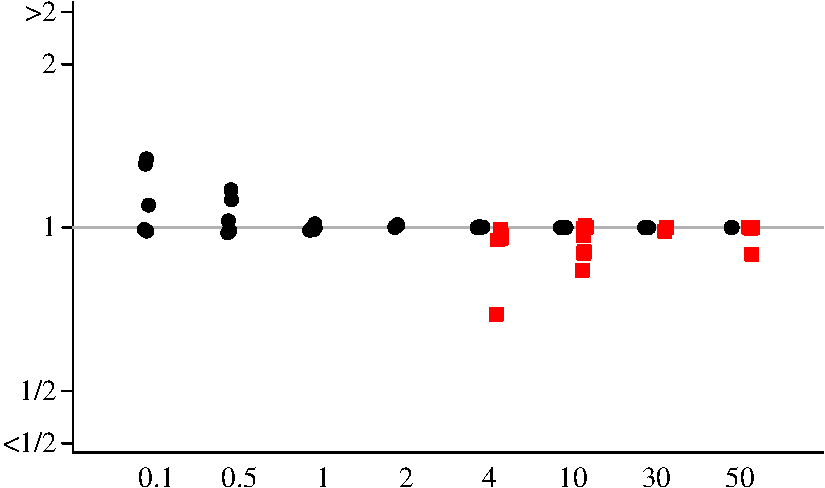
\includegraphics[width=0.45\textwidth]{../figures/graph0.pdf}
\hfill \includegraphics[width=0.45\textwidth]{../figures/{graph0.01}.pdf}\xx \\[15pt]
\xx\hfill Error 5\% \hfill\hfill\hfill Error 10\% \hfill\xx \\
\xx\includegraphics[width=0.45\textwidth]{../figures/{graph0.05}.pdf}
\hfill \includegraphics[width=0.45\textwidth]{../figures/{graph0.1}.pdf}\xx \\

\caption{Comparison of genome coverage estimates obtained by the CovEst E
  model (black circles) and KSA (red squares) on random genomes
  with various coverage levels and error rates. Columns in each plot
  correspond to eight different coverage levels; $y$-axis shows the
  ratio of predicted and real
  coverage on the logarithmic scale. Estimates more than a factor of two
  away from the real value are shown at the top or bottom of the plot.
  For each combination of parameters, we show five replicates. KSA did not
  produce answers for some inputs\cite{covest}. }
\label{fig:covest-ksa-sim}
\end{figure}

\begin{table}[t]
\centerline{
\begin{tabular}{l*{7}{@{\quad}c}}
\toprule
Method   & $c=0.5$ & $c=1$ & $c=2$ & $c=4$ & $c=10$ & $c=30$ & $c=50$ \strut \\
\midrule
CovEst RE & 4.16    &  4.70 & 4.58  &  4.63 & 4.71   & 4.69   & 4.68 \\
KSA      & N/A     & N/A   & N/A   &  6.03 & 4.61   & 4.59   & 4.58 \\
\bottomrule
\end{tabular}}
\caption{Comparison of \emph{E.~coli} genome size estimates (true
  value $4.64$~Mbp) provided by CovEst and KSA at various genome
  coverage values. Estimates are given in Mbp. KSA does not run at low
  coverage\cite{covest}.}
\label{tab:covest-ksa-ecoli}

\end{table}

\todo{treba tu este dake zhrnutie, ci staci ten conclusion co nasleduje?}.

\section{Conclusion}

In this chapter we dealt with a problem of estimating the genome size and the coverage. We showed two main approaches to this problems based on \kmer histogram analysis.

The first approach found in~\cite{waterman} and KSA\cite{williams} was based on precise modeling of repeat content and omitted the error modeling, whereas the second approach was based on precise error modeling and simple repeat modeling.
The first approach works well on high coverage data and is more suitable for genomes, where the repeat content is very different from the simple model in the second approach.

The second approach, which we presented in CovEst\cite{covest}, works well even in very low coverage data ($0.5\times$) or with highly erroneous data ($10\%$ error rate). Our approach is also very universal and easily extensible to more difficult models.

The possibility of estimating the genome size and the coverage from low coverage data is very useful, because obtaining low coverage data is  cheaper than high coverage. Also it is more suitable in large genomes, such as plant genomes where the sizes are in tens of gigabases, where in addition to expensive cost of high coverage sequencing, it would be very time consuming to analyze such amount of data.
